\chapter{Perancangan}
\label{chap:design}

Berdasarkan analisa dari bab 3, pada bab ini akan dibahas mengenai perancangan diagram kelas, dan perancangan antarmuka dari
program.

\section{Perancangan Diagram Kelas}
Berdasarkan hasil analisis dari bab 3, telah dijelaskan pemodelan struktur kelas yang akan digunakan pada program, selanjutnya pada subbab ini merupakan terjemahan dari pemodelan kelas dalam bentuk rancangan diagram kelas pada gambar ~\ref{fig:pemodelan-kelas}.   
\begin{figure}[H]
	\centering
	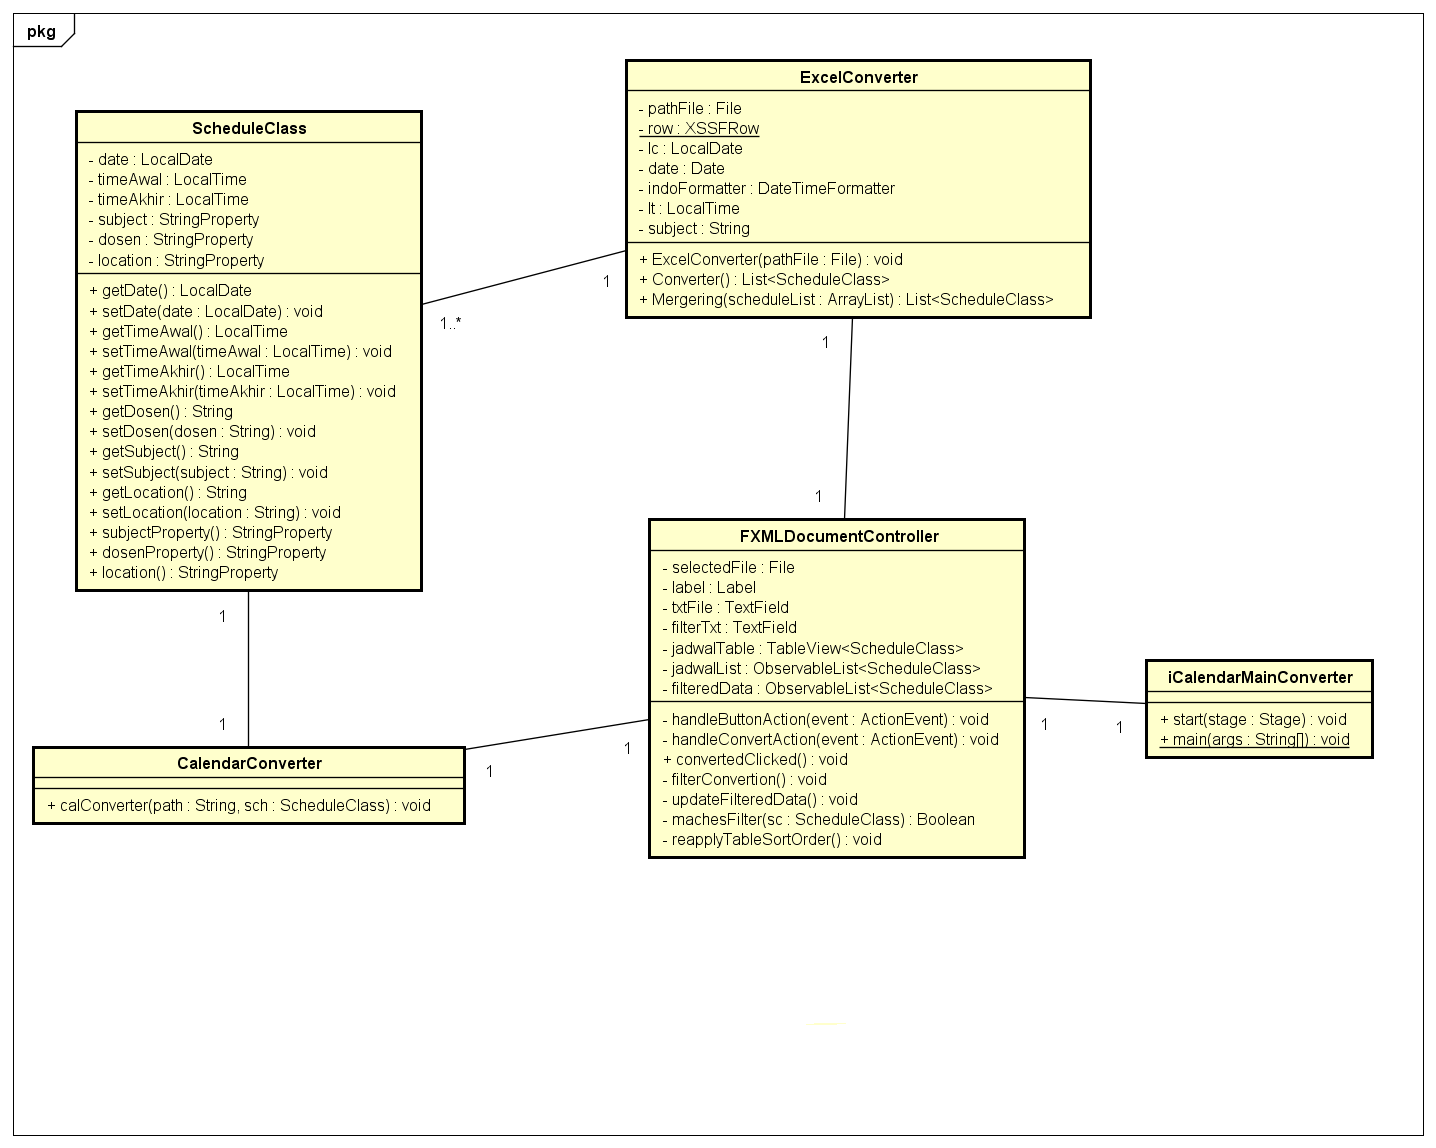
\includegraphics[scale=0.4]{Gambar/kelas-diagram}
	\caption{Gambar Kelas Diagram}
	\label{fig:pemodelan-kelas}
\end{figure}

Berikut ini rincian kelas pada diagram kelas yang tercantum dalam tabel-tabel dibawah ini :

\begin{table}[H]
	\centering
		\caption{Tabel Kelas \textit{ScheduleClass}}
		\label{tab:schedule_class}
		\begin{tabular}{ | c | c | c |}
			\hline
				\multicolumn{3}{|c|}{Atribut} \\ \hline 
				Nama atribut & Tipe Data  & Fungsi \\ \hline
				\textbf{date} & LocalDate & Atribut tanggal\\ \hline
				\textbf{timeAwal} & LocalTime & Atribut jam ujian dimulai\\ \hline
				\textbf{timeAkhir} & LocalTime & Atribut jam ujian berakhir\\ \hline
				\textbf{subject} & StringProperty & Atribut mata kuliah\\ \hline
				\textbf{dosen} & StringProperty & Atribut nama dosen\\ \hline
				\textbf{location} & StringProperty & Atribut lokasi ujian\\ \hline
				\multicolumn{3}{|c|}{Method} \\ \hline
				\multicolumn{2}{|c|}{Nama Method} & Fungsi \\ \hline
				\multicolumn{2}{|l|}{\textbf{getDate()}} & Mendapatkan tanggal\\ \hline
				\multicolumn{2}{|l|}{\textbf{setDate(date: LocalDate)}} & Set tanggal \\ \hline
				\multicolumn{2}{|l|}{\textbf{getTimeAwal()}} & Mendapatkan jam awal ujian \\ \hline
				\multicolumn{2}{|l|}{\textbf{setTimeAwal(timeAwal: LocalTime)}} & Set jam awal ujian\\ \hline
				\multicolumn{2}{|l|}{\textbf{getTimeAkhir()}} & Mendapatkan jam akhir ujian\\ \hline
				\multicolumn{2}{|l|}{\textbf{setTimeAkhir(timeAkhir: LocalTime)}} & Set jam akhir ujian\\ \hline
				\multicolumn{2}{|l|}{\textbf{getDosen()}} & Mendapatkan nama dosen\\ \hline
				\multicolumn{2}{|l|}{\textbf{setDosen(dosen: String)}} & Set nama dosen\\ \hline
				\multicolumn{2}{|l|}{\textbf{getSubject()}} & Mendapatkan nama mata kuliah\\ \hline
				\multicolumn{2}{|l|}{\textbf{setSubject(subject: String)}}& Set mata kuliah \\ \hline
				\multicolumn{2}{|l|}{\textbf{getLocation()}} & Mendapatkan lokasi ujian\\ \hline
				\multicolumn{2}{|l|}{\textbf{setLocation(location: String)}} & Set lokasi ujian\\ \hline
				\multicolumn{2}{|l|}{\textbf{subjectProperty()}} & Mendapatkan properti mata kuliah\\ \hline
				\multicolumn{2}{|l|}{\textbf{dosenProperty()}} & Mendapatkan properti dosen\\ \hline
				\multicolumn{2}{|l|}{\textbf{location()}} & Mendapatkan properti lokasi\\ \hline
		\end{tabular}
\end{table}

\begin{table}[H]
	\centering
		\caption{Tabel Kelas \textit{ExcelConverter}}
		\label{tab:excel_converter}
		\begin{tabular}{ | c | c | p{4cm} |}
			\hline
				\multicolumn{3}{|c|}{Atribut} \\ \hline 
				Nama atribut & Tipe Data  & Fungsi \\ \hline
				\textbf{pathFile} & File & Atribut path file excel mengawas\\ \hline
				\textbf{row} & XSSFRow & Atribut baris dari Excel\\ \hline
				\textbf{lc} & LocalDate & Atribut tanggal ujian\\ \hline
				\textbf{indoFormater} & DateTimeFormatter & Atribut konversi ke zona waktu jakarta\\ \hline
				\textbf{lt} & LocalTime & Atribut jam ujian\\ \hline
				\textbf{subject} & String & Atribut matakuliah\\ \hline
				\multicolumn{3}{|c|}{Method} \\ \hline
				\multicolumn{2}{|c|}{Nama Method} & Fungsi \\ \hline
				\multicolumn{2}{|c|}{\textbf{ExcelConverter(path: File)}} & Konstruktor untuk mendapatkan path file dari excel mengawas ujian\\ \hline
				\multicolumn{2}{|c|}{\textbf{Converter()}} & Konversi excel menjadi list scheduleClass \\ \hline
				\multicolumn{2}{|c|}{\textbf{Mergering(scheduleList: ArrayList)}} & Mengabungkan duplikat entri mengawas dosen \\ \hline
		\end{tabular}
\end{table}

\begin{table}[H]
	\centering
		\caption{Tabel Kelas \textit{CalendarConverter}}
		\label{tab:excel_converter}
		\begin{tabular}{ | c | c | p{4cm} |}
			\hline
				\multicolumn{3}{|c|}{Method}\\ \hline
				\multicolumn{2}{|c|}{Nama Method} & Fungsi \\ \hline
				\multicolumn{2}{|c|}{\textbf{calConverter(path: String, sch: ScheduleClass)}} & Mengkonversi scheduleClass yang dipilih kedalam iCal dan menyimpannya pada path yang ditentukan\\ \hline
		\end{tabular}
\end{table}

\begin{table}[H]
	\centering
		\caption{Tabel Kelas \textit{FXMLDocumentController}}
		\label{tab:FXMLDocumentController}
		\begin{tabular}{ | c | c | p{4cm} |}
			\hline
				\multicolumn{3}{|c|}{Atribut} \\ \hline 
				Nama atribut & Tipe Data  & Fungsi \\ \hline
				\textbf{selectedFile} & File & Atribut file yang dipilih pengguna\\ \hline
				\textbf{label} & Label & Atribut label\\ \hline
				\textbf{txtFile} & TextField & Atribut menampilkan path file yang dipilih\\ \hline
				\textbf{filterTxt} & TextField & Atribut untuk menampilkan filter teks\\ \hline
				\textbf{jadwalTable} & TableView<ScheduleClass> & Atribut menampilkan tabel jadwal\\ \hline
				\textbf{jadwalList} & ObservableList<ScheduleClass> & Atribut untuk menyimpan jadwal\\ \hline
				\textbf{filteredData} & ObservableList<ScheduleClass> & Atribut untuk menyimpan data yang telah di filter\\ \hline
				\multicolumn{3}{|c|}{Method} \\ \hline
				\multicolumn{2}{|c|}{Nama Method} & Fungsi \\ \hline
				\multicolumn{2}{|c|}{\textbf{handleButtonAction(event: ActionEvent)}} & Method untuk melakukan browse dan mendapatkan file excel\\ \hline
				\multicolumn{2}{|c|}{\textbf{handleConvertAction(event: ActionEvent)}} & Method untuk membaca file excel \\ \hline
				\multicolumn{2}{|c|}{\textbf{convertedClicked()}} & Method untuk konversi \textit{selected item} menjadi iCal  \\ \hline
				\multicolumn{2}{|c|}{\textbf{filterConvertion()}} & Method untuk menerima masukan filter dari pengguna \\ \hline
				\multicolumn{2}{|c|}{\textbf{updateFilteredData()}} & Menginisiasi list filteredData \\ \hline
				\multicolumn{2}{|c|}{\textbf{matchesFilter(sc: ScheduleClass)}} & Mencocokan nama dosen sesuai yang di inginkan pengguna \\ \hline
				\multicolumn{2}{|c|}{\textbf{reapplyTableSortOrder()}} & Mengatur urutan tabel setelah di filter \\ \hline
		\end{tabular}
\end{table}

\begin{table}[H]
	\centering
		\caption{Tabel Kelas \textit{iCalendarMainConverter}}
		\label{tab:iCalendarMainConverter}
		\begin{tabular}{ | c | c | p{4cm} |}
			\hline
				\multicolumn{3}{|c|}{Method}  \\ \hline
				\multicolumn{2}{|c|}{Nama Method} & Fungsi \\ \hline
				\multicolumn{2}{|c|}{\textbf{start(stage: Stage)}} & Menampilkan window\\ \hline
			\multicolumn{2}{|c|}{\textbf{main(args: String[])}} & Mengeksekusi program\\ \hline
		\end{tabular}
\end{table}

\section{Perancangan Antarmuka}
Setelah melalui serangkaian anlisis dan perancangan diagram kelas pada sub bab ini akan dijelaskan mengenai gambaran bentuk program mengawas ujian tersebut.

\begin{enumerate}
	\item Halaman awal program\\
	Ini adalah tampilan awal pada saat pengguna pertama kali menjalankan program.		
	\begin{figure}[H]
		\centering
		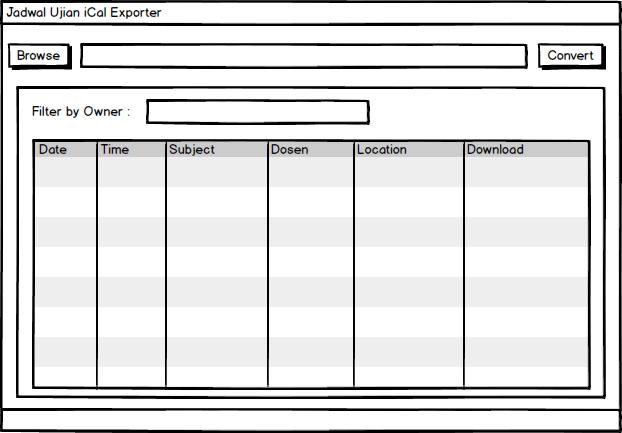
\includegraphics[scale=0.5]{Gambar/antarmuka}
		\caption{Tampilan awal Program}
		\label{fig:tampilan_awal}
		\end{figure}
		
		Pada gambar ~\ref{fig:tampilan_awal} terdapat beberapa \textit{button} dan \textit{textbox} yang memiliki fungsi sebagai berikut.
		\begin{itemize}
			\item \textit{}{Browse} : berfungsi untuk membuka \textit{pop-up window} sebagai sarana pengguna memilih file excel yang akan dimasukkan.
			\item \textit{Textbox path} : alamat file yang telah dipilih oleh pengguna akan dicatat pada \textit{textbox} ini.
			\item \textit{Convert} : tombol ini berfungsi mengeksekusi program untuk membaca file yang telah dimasukkan oleh pengguna.
			\item \textit{Textbox filter} : merupakan fitur untuk memfilter jadwal mengawas berdasarkan nama dosen yang sesuai dengan \textit{input} pengguna.
			\item \textit{TableView} : jadwal yang telah dibaca pada excel selanjutnya akan ditampilkan pada tabel ini. tabel ini terdiri dari kolom tanggal, waktu, matakuliah, dosen, lokasi, dan \textit{download} untuk mengunduh file iCal.		
		\end{itemize}
	\item Halaman untuk melakukan \textit{Browse} file excel\\
	Halaman ini merupakan halaman dimana pengguna melakukan pemilihan \textit{input} file excel jadwal mengawas. Halaman \textit{browser} menyesuaikan tipe sistem operasi yang dipakai.
		\begin{figure}[H]
		\centering
		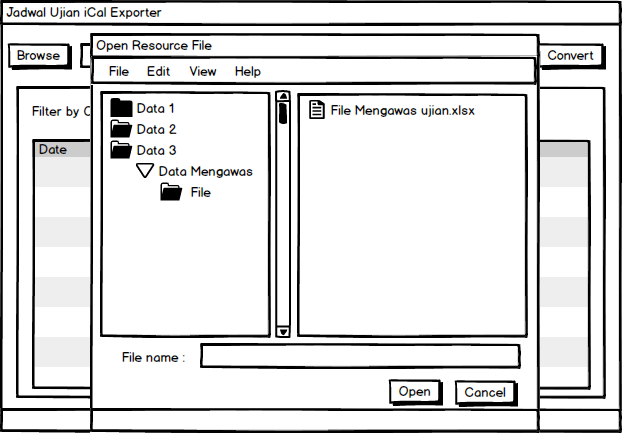
\includegraphics[scale=0.5]{Gambar/antarmuka3}
		\caption{Tampilan \textit{Browse} file excel}
		\label{fig:browse}
		\end{figure}
	\item Halaman setelah excel dibaca\\
	Halaman ini menujukan ketika file excel telah sukses dibaca dan ditampilkan pada \textit{tableview}.
		\begin{figure}[H]
		\centering
		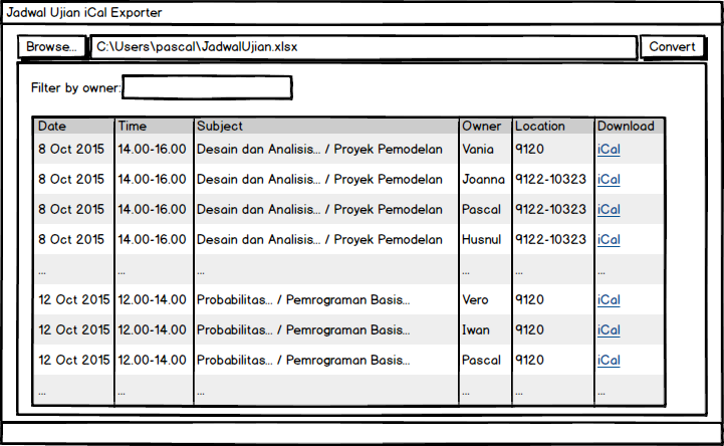
\includegraphics[scale=0.5]{Gambar/antarmuka2}
		\caption{Tampilan setelah excel dibaca}
		\label{fig:excel_dibaca}
		\end{figure}
	\item Halaman untuk menyimpan iCal\\
	Halaman ini dimana pengguna telah memilih salah satu jadwal dan akan menyimpannya dalam betuk iCal. Halaman \textit{save} menyesuaikan sistem operasi yang dipakai. 
		\begin{figure}[H]
		\centering
		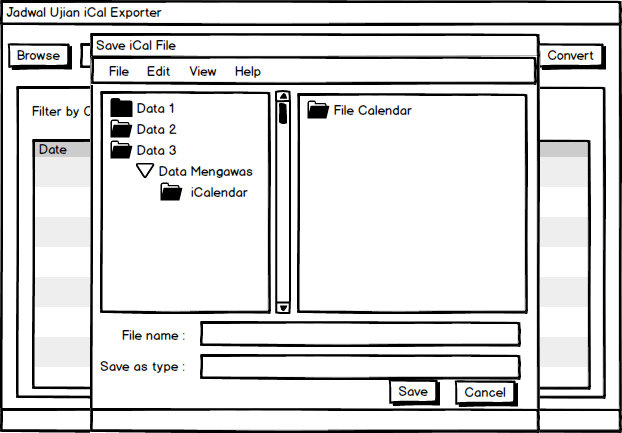
\includegraphics[scale=0.5]{Gambar/antarmuka4}
		\caption{Tampilan untuk menyimpan iCal}
		\label{fig:jadwalpng}
		\end{figure}
\end{enumerate}

\section{Rancangan \textit{Method-Method} Utama}
Berikut ini adalah rancangan \textit{method} utama program jadwal mengawas ujian yang berperan penting dalam perangkat lunak:
\begin{enumerate}
	\item Converter() - ExcelConverter\\
	\begin{tabular}{l c p{9cm}}
		Input & : & - \\ 
		Output & : & List<ScheduleClass>  \\ 
		Deskripsi & : & Method ini membaca excel yang di \textit{input} oleh pengguna dan mengkonversikannya kedalam bentuk list.\\
		Algoritma & : & \begin{enumerate}
			\item Ambil path file yang telah di \textit{input} oleh pengguna.
			\item Cari kolom No. pada file excel dan jadikan acuan bahwa program akan membaca setelah dari index kolom tersebut.
			\item Baca baris per baris namun cek terlebih dahulu apakah di kolom No. baris tersebut masih berupa nomer, apabila tidak maka berhenti membaca karena baris yang berisi jadwal sudah terbaca semua.
			\item Cek apakah baris mengandung kata \textit{LIBUR} bila ya maka lewati saja.
			\item Pisahkan hari dan tanggal lalu konversi menjadi LocalDate. 
			\item Pisahkan jam menjadi jamAwal dan jamAkhir, lalu konversi menjadi LocalTime.
			\item jika menemukan kata \textit{Shift} atau \textit{Lab} maka lokasi ujian adalah Lab.
			\item Masukan semua kedalam sebuah ArrayList<ScheduleClass>.
		\end{enumerate}
		\end{tabular}	
	
	\item Mergering() - ExcelConverter\\
	\begin{tabular}{l c p{9cm}}
		Input & : & List<ScheduleClass> \\ 
		Output & : & List<ScheduleClass> \\ 
		Deskripsi & : & Method ini menghapus \textit{entry} duplikat dari dosen yang mempunyai dua jadwal mengawas pada hari yang sama.\\
		Algoritma & : & 
			\begin{enumerate}
				\item Cari subject/mata kuliah yang tidak memiliki dosen pada ArrayList yang telah di proses oleh \textit{method} Convert() karena bila program membaca kolom yang di-\textit{merger} maka hanya kolom pertama saja yang dibaca sehingga kolom keduanya kosong.
				\item Masukan baris yang tidak memiliki dosen kedalam ArrayList baru.
				\item Hapus baris yang tidak memiliki dosen pada ArrayList master.
				\item Cocokan waktu dan tanggal ujian ArrayList master dengan temp, bila sama maka tambahkan matakuliah/subject pada ArrayList master.
			\end{enumerate}
		\end{tabular}	
	
	\item calConverter() - CalendarConverter\\
	\begin{tabular}{l c p{9cm}}
		Input & : & sch: ScheduleClass , path: String\\ 
		Output & : & void \\ 
		Deskripsi & : & Method ini mengkonversi ScheduleClass menjadi iCal\\
		Algoritma & : & 
			\begin{enumerate}
				\item Inisiasi variable zona waktu Indonesia.
				\item Konversi tanggal, bulan, dan tahun kedalam GregorianCalender.
				\item Masukan event berdasarkan subject/mata kuliah , lokasi, dan dosen yang mengawas.
				\item Inisiasi kalender dan masukan variable tanggal dan event yang telah dibuat sebelumnya kedalam variable kalender tersebut.
				\item Simpan pada path yang telah di pilih oleh pengguna.
			\end{enumerate}
		\end{tabular}	
		
	\item filterConvertion() - FXMLDocumentController\\
	\begin{tabular}{l c p{9cm}}
		Input & : & void\\ 
		Output & : & void \\ 
		Deskripsi & : & Method ini menjalankan filter data dosen sesuai \textit{input} pengguna\\
		Algoritma & : & 
			\begin{enumerate}
				\item Inisiasi tabel dengan list yang sudah di filter.
				\item Masukan nilai yang sama kedalam list filter jika dosen yang dicari sesuai dengan \textit{input} pengguna.
				\item Atur kembali urutan tabel pada perangkat lunak.
			\end{enumerate}
		\end{tabular}	
\end{enumerate}
